%  LaTeX support: latex@mdpi.com 
%  For support, please attach all files needed for compiling as well as the log file, and specify your operating system, LaTeX version, and LaTeX editor.

%=================================================================
\documentclass[journal,article,submit,pdftex,moreauthors]{Definitions/mdpi} 
\usepackage{pythontex}
% For posting an early version of this manuscript as a preprint, you may use "preprints" as the journal and change "submit" to "accept". The document class line would be, e.g., \documentclass[preprints,article,accept,moreauthors,pdftex]{mdpi}. This is especially recommended for submission to arXiv, where line numbers should be removed before posting. For preprints.org, the editorial staff will make this change immediately prior to posting.

%--------------------
% Class Options:
%--------------------
%----------
% journal
%----------
% Choose between the following MDPI journals:
% acoustics, actuators, addictions, admsci, adolescents, aerospace, agriculture, agriengineering, agronomy, ai, algorithms, allergies, alloys, analytica, animals, antibiotics, antibodies, antioxidants, applbiosci, appliedchem, appliedmath, applmech, applmicrobiol, applnano, applsci, aquacj, architecture, arts, asc, asi, astronomy, atmosphere, atoms, audiolres, automation, axioms, bacteria, batteries, bdcc, behavsci, beverages, biochem, bioengineering, biologics, biology, biomass, biomechanics, biomed, biomedicines, biomedinformatics, biomimetics, biomolecules, biophysica, biosensors, biotech, birds, bloods, blsf, brainsci, breath, buildings, businesses, cancers, carbon, cardiogenetics, catalysts, cells, ceramics, challenges, chemengineering, chemistry, chemosensors, chemproc, children, chips, cimb, civileng, cleantechnol, climate, clinpract, clockssleep, cmd, coasts, coatings, colloids, colorants, commodities, compounds, computation, computers, condensedmatter, conservation, constrmater, cosmetics, covid, crops, cryptography, crystals, csmf, ctn, curroncol, currophthalmol, cyber, dairy, data, dentistry, dermato, dermatopathology, designs, diabetology, diagnostics, dietetics, digital, disabilities, diseases, diversity, dna, drones, dynamics, earth, ebj, ecologies, econometrics, economies, education, ejihpe, electricity, electrochem, electronicmat, electronics, encyclopedia, endocrines, energies, eng, engproc, ent, entomology, entropy, environments, environsciproc, epidemiologia, epigenomes, est, fermentation, fibers, fintech, fire, fishes, fluids, foods, forecasting, forensicsci, forests, foundations, fractalfract, fuels, futureinternet, futureparasites, futurepharmacol, futurephys, futuretransp, galaxies, games, gases, gastroent, gastrointestdisord, gels, genealogy, genes, geographies, geohazards, geomatics, geosciences, geotechnics, geriatrics, hazardousmatters, healthcare, hearts, hemato, heritage, highthroughput, histories, horticulturae, humanities, humans, hydrobiology, hydrogen, hydrology, hygiene, idr, ijerph, ijfs, ijgi, ijms, ijns, ijtm, ijtpp, immuno, informatics, information, infrastructures, inorganics, insects, instruments, inventions, iot, j, jal, jcdd, jcm, jcp, jcs, jdb, jeta, jfb, jfmk, jimaging, jintelligence, jlpea, jmmp, jmp, jmse, jne, jnt, jof, joitmc, jor, journalmedia, jox, jpm, jrfm, jsan, jtaer, jzbg, kidney, kidneydial, knowledge, land, languages, laws, life, liquids, literature, livers, logics, logistics, lubricants, lymphatics, machines, macromol, magnetism, magnetochemistry, make, marinedrugs, materials, materproc, mathematics, mca, measurements, medicina, medicines, medsci, membranes, merits, metabolites, metals, meteorology, methane, metrology, micro, microarrays, microbiolres, micromachines, microorganisms, microplastics, minerals, mining, modelling, molbank, molecules, mps, msf, mti, muscles, nanoenergyadv, nanomanufacturing, nanomaterials, ncrna, network, neuroglia, neurolint, neurosci, nitrogen, notspecified, nri, nursrep, nutraceuticals, nutrients, obesities, oceans, ohbm, onco, oncopathology, optics, oral, organics, organoids, osteology, oxygen, parasites, parasitologia, particles, pathogens, pathophysiology, pediatrrep, pharmaceuticals, pharmaceutics, pharmacoepidemiology, pharmacy, philosophies, photochem, photonics, phycology, physchem, physics, physiologia, plants, plasma, pollutants, polymers, polysaccharides, poultry, powders, preprints, proceedings, processes, prosthesis, proteomes, psf, psych, psychiatryint, psychoactives, publications, quantumrep, quaternary, qubs, radiation, reactions, recycling, regeneration, religions, remotesensing, reports, reprodmed, resources, rheumato, risks, robotics, ruminants, safety, sci, scipharm, seeds, sensors, separations, sexes, signals, sinusitis, skins, smartcities, sna, societies, socsci, software, soilsystems, solar, solids, sports, standards, stats, stresses, surfaces, surgeries, suschem, sustainability, symmetry, synbio, systems, taxonomy, technologies, telecom, test, textiles, thalassrep, thermo, tomography, tourismhosp, toxics, toxins, transplantology, transportation, traumacare, traumas, tropicalmed, universe, urbansci, uro, vaccines, vehicles, venereology, vetsci, vibration, viruses, vision, waste, water, wem, wevj, wind, women, world, youth, zoonoticdis 

%---------
% article
%---------
% The default type of manuscript is "article", but can be replaced by: 
% abstract, addendum, article, book, bookreview, briefreport, casereport, comment, commentary, communication, conferenceproceedings, correction, conferencereport, entry, expressionofconcern, extendedabstract, datadescriptor, editorial, essay, erratum, hypothesis, interestingimage, obituary, opinion, projectreport, reply, retraction, review, perspective, protocol, shortnote, studyprotocol, systematicreview, supfile, technicalnote, viewpoint, guidelines, registeredreport, tutorial
% supfile = supplementary materials

%----------
% submit
%----------
% The class option "submit" will be changed to "accept" by the Editorial Office when the paper is accepted. This will only make changes to the frontpage (e.g., the logo of the journal will get visible), the headings, and the copyright information. Also, line numbering will be removed. Journal info and pagination for accepted papers will also be assigned by the Editorial Office.

%------------------
% moreauthors
%------------------
% If there is only one author the class option oneauthor should be used. Otherwise use the class option moreauthors.

%---------
% pdftex
%---------
% The option pdftex is for use with pdfLaTeX. If eps figures are used, remove the option pdftex and use LaTeX and dvi2pdf.

%=================================================================
% MDPI internal commands
\firstpage{1} 
\makeatletter 
\setcounter{page}{\@firstpage} 
\makeatother
\pubvolume{1}
\issuenum{1}
\articlenumber{0}
\pubyear{2022}
\copyrightyear{2022}
%\externaleditor{Academic Editor: Firstname Lastname}
\datereceived{} 
%\daterevised{} % Only for the journal Acoustics
\dateaccepted{} 
\datepublished{} 
%\datecorrected{} % Corrected papers include a "Corrected: XXX" date in the original paper.
%\dateretracted{} % Corrected papers include a "Retracted: XXX" date in the original paper.
\hreflink{https://doi.org/} % If needed use \linebreak
%\doinum{}
%------------------------------------------------------------------
% The following line should be uncommented if the LaTeX file is uploaded to arXiv.org
%\pdfoutput=1

%=================================================================
% Add packages and commands here. The following packages are loaded in our class file: fontenc, inputenc, calc, indentfirst, fancyhdr, graphicx, epstopdf, lastpage, ifthen, lineno, float, amsmath, setspace, enumitem, mathpazo, booktabs, titlesec, etoolbox, tabto, xcolor, soul, multirow, microtype, tikz, totcount, changepage, attrib, upgreek, cleveref, amsthm, hyphenat, natbib, hyperref, footmisc, url, geometry, newfloat, caption

%=================================================================
%% Please use the following mathematics environments: Theorem, Lemma, Corollary, Proposition, Characterization, Property, Problem, Example, ExamplesandDefinitions, Hypothesis, Remark, Definition, Notation, Assumption
%% For proofs, please use the proof environment (the amsthm package is loaded by the MDPI class).

%=================================================================
% Full title of the paper (Capitalized)
\Title{Using Particle Filter to Solve the Problem of Symmetric Multiple Solutions in Inverse Kinematics of Manipulator}

% MDPI internal command: Title for citation in the left column
\TitleCitation{Title}

% Author Orchid ID: enter ID or remove command
\newcommand{\orcidauthorA}{0000-0000-0000-000X} % Add \orcidA{} behind the author's name
%\newcommand{\orcidauthorB}{0000-0000-0000-000X} % Add \orcidB{} behind the author's name

% Authors, for the paper (add full first names)
\Author{Chien-Lin Chiang $^{1,}$ Chang-Chen Hsieh $^{2,}$ Mao-Hung Yang $^{3,}$I-Long Lin $^{4,}$and Yi-Yuan Chiang $^{5,}$*}

%\longauthorlist{yes}

% MDPI internal command: Authors, for metadata in PDF
\AuthorNames{Chien-Lin Chiang,Chang-Chen Hsieh,Mao-Hung Yang, I-Long Lin and Yi-Yuan Chiang}

% MDPI internal command: Authors, for citation in the left column
\AuthorCitation{Lastname, F.; Lastname, F.; Lastname, F.}
% If this is a Chicago style journal: Lastname, Firstname, Firstname Lastname, and Firstname Lastname.

% Affiliations / Addresses (Add [1] after \address if there is only one affiliation.)
\address{%
$^{1}$ \quad Tatung University; f2267505@gmail.com\\
$^{2}$ \quad Vanung University; superlongtw@gmail.com\\
$^{3}$ \quad Vanung University; 0309.kevin@gmail.com\\
$^{4}$ \quad Tatung University; cyberpaul@ttu.edu.tw\\
$^{5}$ \quad Vanung University; yychiang.vnu@gmail.com}

% Contact information of the corresponding author
\corres{Correspondence: yychiang.vnu@gmail.com; Tel.: +886-925-688317}

% Current address and/or shared authorship
\firstnote{} 
\secondnote{}
% The commands \thirdnote{} till \eighthnote{} are available for further notes

%\simplesumm{} % Simple summary

%\conference{} % An extended version of a conference paper

% Abstract (Do not insert blank lines, i.e. \\) 
\abstract{In the inverse kinematics of robotic arm, the most frequently encountered problem is multiple solutions for the poses of the arm. The multiple solutions often appear symmetrically. In practical applications, a set of solutions must be selected from the multiple solutions as the pose of the robot arm. The symmetric multiple solutions are all reasonable poses reachable by the robot arm. However, in the process of arm movement, if the solution is not selected properly, the robotic arm will rapidly change from a solution to a solution in two adjacent time samples. The posture of the symmetric solution sampled at the previous time will cause the mechanical arm to change the posture rapidly and cause damage to the mechanism, and even cause the mechanism to oscillate greatly. To avoid the interference of symmetric multiple solutions, we adopt the non-parametric Bayesian filter (that is, particle filter) based on the Monte Carlo method to process the robotic arm instead of the traditional inverse kinematics method using algebraic or geometric methods. The particle filter uses many random sample points and the design of importance weights to make the sample points converge to the optimal solution in an iterative process. This paper shows how to use the design of importance weights to prevent the oscillation problem of symmetrical multiple solutions in adjacent time sampling during the movement of the manipulator.}

% Keywords
\keyword{mechanical arm; inverse kinematics; multiple solutions; symmetry} 

% The fields PACS, MSC, and JEL may be left empty or commented out if not applicable
%\PACS{J0101}
%\MSC{}
%\JEL{}

%%%%%%%%%%%%%%%%%%%%%%%%%%%%%%%%%%%%%%%%%%
% Only for the journal Diversity
%\LSID{\url{http://}}

%%%%%%%%%%%%%%%%%%%%%%%%%%%%%%%%%%%%%%%%%%
% Only for the journal Applied Sciences
%\featuredapplication{Authors are encouraged to provide a concise description of the specific application or a potential application of the work. This section is not mandatory.}
%%%%%%%%%%%%%%%%%%%%%%%%%%%%%%%%%%%%%%%%%%

%%%%%%%%%%%%%%%%%%%%%%%%%%%%%%%%%%%%%%%%%%
% Only for the journal Data
%\dataset{DOI number or link to the deposited data set if the data set is published separately. If the data set shall be published as a supplement to this paper, this field will be filled by the journal editors. In this case, please submit the data set as a supplement.}
%\datasetlicense{License under which the data set is made available (CC0, CC-BY, CC-BY-SA, CC-BY-NC, etc.)}

%%%%%%%%%%%%%%%%%%%%%%%%%%%%%%%%%%%%%%%%%%
% Only for the journal Toxins
%\keycontribution{The breakthroughs or highlights of the manuscript. Authors can write one or two sentences to describe the most important part of the paper.}

%%%%%%%%%%%%%%%%%%%%%%%%%%%%%%%%%%%%%%%%%%
% Only for the journal Encyclopedia
%\encyclopediadef{For entry manuscripts only: please provide a brief overview of the entry title instead of an abstract.}

%%%%%%%%%%%%%%%%%%%%%%%%%%%%%%%%%%%%%%%%%%
% Only for the journal Advances in Respiratory Medicine
%\addhighlights{yes}
%\renewcommand{\addhighlights}{%

%\noindent This is an obligatory section in “Advances in Respiratory Medicine”, whose goal is to increase the discoverability and readability of the article via search engines and other scholars. Highlights should not be a copy of the abstract, but a simple text allowing the reader to quickly and simplified find out what the article is about and what can be cited from it. Each of these parts should be devoted up to 2~bullet points.\vspace{3pt}\\
%\textbf{What are the main findings?}
% \begin{itemize}[labelsep=2.5mm,topsep=-3pt]
% \item First bullet.
% \item Second bullet.
% \end{itemize}\vspace{3pt}
%\textbf{What is the implication of the main finding?}
% \begin{itemize}[labelsep=2.5mm,topsep=-3pt]
% \item First bullet.
% \item Second bullet.
% \end{itemize}
%}

%%%%%%%%%%%%%%%%%%%%%%%%%%%%%%%%%%%%%%%%%%
\begin{document}

%%%%%%%%%%%%%%%%%%%%%%%%%%%%%%%%%%%%%%%%%%
%\setcounter{section}{-1} %% Remove this when starting to work on the template.
\section{Introduction}

In today's society, after entering the industrial era 4.0, robotic arms have become an indispensable and important piece of equipment in many heavy industries today. In many applications, robotic arm has its important contribution, especially in many semi-automatic or even fully automatic factories. The application field is also very wide, automotive, plastics, electronics, chemical, machinery, medical and many other fields, are often seen in the robot arm related applications, especially automated assembly, transport, cutting and welding.
The problem of multiple solutions is often encountered in the inverse kinematics of mechanical arms. The multiple solutions often appear symmetrically. In practical application, a set of solutions must be selected from the multiple solutions as the pose of the robotic arm. Although the symmetric multiple solutions are reasonable poses for the robotic arm, but in the process of arm movement, if the solution is not selected properly, it will make the robotic arm change the pose from a certain solution to the symmetric solution of the previous time in two nearby time samples, which will make the robotic arm change the pose quickly and cause damage to the mechanism, or even cause the mechanism to vibrate significantly. In order to avoid the interference of symmetric multiple solutions, we abandon the traditional algebraic or geometric method of inverse kinematics, and adopt the Monte Carlo-based nonparametric Bayesian filter (also known as particle filter) to deal with the problem of robot arm inverse kinematics. The particle filter is designed with a large number of random sample points and importance weights to allow the sample points to converge to the best solution in an iterative process. In this paper, we illustrate how to use the importance weight design to avoid the oscillation problem of multiple solutions of symmetry in the adjacent time samples during the robot motion.
In the process of industrial automation, we believe that robotics-related industries, including robotic arms, are sure to shine in the future. We also hope to improve the efficiency and quality of robotic arms through this study.


\section{Background Knowledge: Inverse Kinematics}
The purpose of inverse kinematics is to investigate how the end point of a robotic arm reaches a specific position and attitude in space, i.e., given the end point of a bar (Link)  The spatial position of the end point of the link in the absolute coordinate system is derived from the equation to find the rotation angle of each joint. In the process of solving, it is necessary to consider whether the end point  Whether the end point is within the reach of the robot arm (Figure 2-16, 17), the geometric limitation of the arm itself, and whether there is any obstacle in the arm movement. If there are multiple solutions, the solution closest to the current state is chosen [2].

In forward kinematics, we use the known  to find the  In inverse kinematics, we use the known  to find  . Because the inverse kinematics will encounter multiple solutions to the problem, the solution method will be relatively more complicated than the forward one [9].

The solution methods are broadly classified as follows: analytical (geometric, algebraic, etc.) and numerical methods [3][4].

\subsection{Geometric Method}
The geometric methods could be used to solve not only 3D robot arms, but also 2D planar robots. For 3D cases, it just need to separate the 3D space geometry into 2D planar geometry as shown in Figure~\ref{fig1}.

\begin{figure}[H]
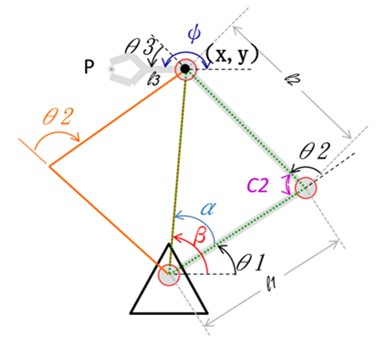
\includegraphics[width=10.5 cm]{Definitions/fig1}
\caption{The schematic of RRR type robot arm.\label{fig1}}
\end{figure}   

The end point of link2 is $(x,y)$. Use the cosine theorem to find $\theta_2$.  The angle could be plotted into two solutions: the green triangle and the orange one. Take Figure~\ref{fig1} as an example, using the geometric method, the space is separated into planar geometry.  Since $l_1$ and $l_2$ are the  lengths of Link1 and Link2, respectively; we could use the cosine theorem to find the $c2$ angle. Therefore, we have the floolwing equations:
\begin{align} 
x^2+y^2&=l_1^2+l_2^2-2l_1l_2\cos(\pi-\theta_2) \\
\cos(\theta_2)&=\frac{x^2+y^2-l_1^2-l_2^2}{2l_1l_2}
\end{align}
Then, $\theta_2$ along with $\theta_1$ and $\theta_3$ could be solved by inverse trigonometric functions.
\subsection{Algebraic Method}
The algebraic method is to directly combine the items in the pose matrix $T_0,T_1,\ldots,T_n$, and to define the intermediate variables (which is a combination of joint parameters). for the purpose of constructing a one-dimensional high-order equation. All joint angles can be find by solving this equation. We use the same example as shown in Figure~\ref{fig1}, the pose matrix of the end point is
\begin{align}
^{0}_{3}T&=
\begin{bmatrix}
\cos(\theta_1+\theta_2+\theta_3) & -\sin(\theta_1+\theta_2+\theta_3) & 0 & l_1\cos\theta_1+l_2\cos(\theta_1+\theta_2) \\
\sin(\theta_1+\theta_2+\theta_3) & \cos(\theta_1+\theta_2+\theta_3) & 0 & l_1\sin\theta_1+l_2\sin(\theta_1+\theta_2) \\
0 & 0 & 1 & 0 \\
0 & 0 & 0 & 1 
\end{bmatrix}\\
&=
\begin{bmatrix}
\cos(\phi) & -\sin(\phi) & 0 & x \\
\sin(\phi) & \cos(\phi) & 0 & y \\
0 & 0 & 1 & 0 \\
0 & 0 & 0 & 1 
\end{bmatrix}.
\end{align}
By (3) and (4), all angles could be solved by simple algebraic computations.
%%%%%%%%%%%%%%%%%%%%%%%%%%%%%%%%%%%%%%%%%%
\section{Particle filter and application in inverse kinematics}
\subsection{Particle filter}
Particle filters are commonly used for robot positioning and tracking applications. In this paper, we use the particles in the particle filter to represent the pose of the robotic arm and the position of the particles to represent the end position of the robotic arm. Thus, each particle can be considered as a robot arm state, and each joint angle is embedded in the particle parameters [5]. A group of particles is used to track the position of the robotic arm branch, and the attitude of the particles is averaged to find the estimated attitude. In this way, the inverse kinematics of the robotic arm can be efficiently calculated.

For a particle filter, a particle is a pair with $n$ variable of $p=(v_1,v_2,\ldots,v_n)$. where $v_i$ is a certain state of the robot. For example, the joint angle and end position of a robot arm; the position coordinates, speed, acceleration, and direction of a self-driving car, etc. Simply put, the particle set here is a set of hundreds, thousands, or tens of thousands of particles, which is what we call the particle filter summary.

Particle filter is a kind of Bayesian filters, specifically, nonparametric Bayesian filters. The Bayesian filter is an algorithm for estimating the state of a robot based on Bayes' theorem in the theory of probability [6]. Before going deeper into the theory, let us first explain the robot's environment. In this paper, we refer to the robot as a multi-joint robot arm. The state of the robot refers to the angle of each joint of the robot arm and the coordinates of the end position of the arm. Observations of sensors, in a broad sense, refer to the readings of any sensors mounted on the robot. In the study of the inverse kinematics of the robot arm, we assume that the current states of each joint, i.e., the current angles, can be read by the internal encoder of the motor. The end position of the robot arm can be indirectly calculated from the angle of each joint and the link length, and is therefore observable. The control variavle is a variable that can be controlled on the robot. Changing the control variables will result in a change in the robot's state. The control variables of the robot arm are the joints of each controllable angle.

\subsection{Design of particle filter in inverse kinematics}
The main purpose of this section is to use the particle filter to deal with the inverse kinematics of the robot arm. The so-called inverse kinematics is to find an attitude under the condition that the end coordinates of the robot arm are known, so that the end coordinates of the robot arm under the attitude can meet the condition. The attitude of the robot arm is determined by all the joint angles together. Therefore, in more detail, the so-called inverse kinematics is to derive the angle of each joint from the known terminal coordinates, so that the terminal coordinates of the robot arm can meet the required conditions under the attitude.

\begin{figure}[H]
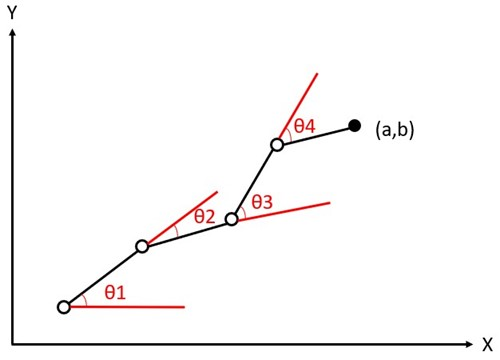
\includegraphics[width=10.5 cm]{Definitions/fig2}
\caption{Four joints robot arm.\label{fig2}}
\end{figure}   

In Figure~\ref{fig2}, we have marked the joint angles. The angle of each joint is calculated from the extension of the previous bar to the angle of the bar of the joint. The first joint is calculated from the horizontal line to the angle of the first bar, since there is no previous bar. The attitude of the robot arm is defined as  . The so-called example in the particle filter, as applied to the inverse kinematics of the robot arm, refers to a specific posture. As we described in the previous section, particle filters are generally used in robot positioning and tracking problems. In inverse kinematics, we have to invert the pose of a robot arm from a known terminal coordinate, which is actually very similar to the concept of localization and tracking. We can consider the process of to find the appropriate attitude of the robot arm as a localization problem, that is, to find out the position of the attitude. On the other hand, we can also consider this problem as a tracking problem, where the target pose is the state we want to track [11].

After understanding how to correspond the inverse kinematics with the particle filter, we will explain the details of the particle filter algorithm.

\subsubsection{Step 1: Random particle generation}
The first step of the algorithm is to randomly generate particles. Suppose we want to generate  particles, these  particles represent  different poses of the robot arm. The following symbols are used to represent  particles.
\begin{align}
(\theta_1^{(1)},\theta_2^{(1)},\theta_3^{(1)},\theta_4^{(1)})
\end{align}
\begin{align*}
(\theta_1^{(2)},\theta_2^{(2)},\theta_3^{(2)},\theta_4^{(2)})\\
\vdots \\
(\theta_1^{(n)},\theta_2^{(n)},\theta_3^{(n)},\theta_4^{(n)})
\end{align*}
The lower number represents the number of joint angles, while the upper number represents the number of particles.

\subsubsection{Step 2: Calculate importance weights}
After the random particle generation, the next step is to calculate the weight of each particle. The weight of the particle represents the good or bad of the example, so in order to calculate the weight, we need to find the error of the particle first. To calculate the error, we have to use the robot arm's forward kinematics to obtain a terminal coordinate from the particle's joint assembly, $(x^{(i)},y^{(i)})$, and then use the distance between the calculated terminal coordinates and the actual terminal coordinates $(x_0,y_0)$. The distance between the calculated terminal coordinates and the actual terminal coordinates is used as the error function. After the error is obtained, the weight can be further calculated. In the following, we explain the above steps in detail.

Each particle represents a certain attitude from which an end coordinate can be calculated using the forward kinematics. The forward kinematics can be considered as a function (FK). Then,
$$(x^{(i)},y^{(i)})=FK(\theta_1^{(i)},\theta_2^{(i)},\theta_3^{(i)},\theta_4^{(i)})$$

The distance is calculated using the usual Euclidean distance,  $d^{(i)}$, represents the distance from the first particle to $(x_0, y_0)$. The distance,
\begin{align}
d^{(i)}=\sqrt{(x^{(i)}-x_0)^2+(y^{(i)}-y_0)^2}
\end{align}

Once we have the distance, we can convert the distance to a weight in the following way.

$$w^{(i)}=\frac{1}{1+d^{(i)}}$$

In order to deepen the difference between good and bad particles, the above weights can be taken as  times. As for how many times, it must be decided in the experiment.


\subsubsection{Step 3: Resampling}
The weight of each particle calculated in the previous step will be used as the basis for resampling. We convert the weights into probabilities, and then use the probabilities to resample the particles. Therefore, the higher the weight of a particle, the more often it will be selected after resampling.
First, each weight must go through a formalization process before it can be converted into a probability.
Define
$$W=\Sigma_{i=1}^{n}w^{(n)}.$$
Then,
\begin{align}
\overline{w}^{(i)}=\frac{w^{(i)}}{W}=p^{(i)}
\end{align}
The probability here will be the probability that the particle will be selected after resampling. In order to keep the number of particles from decreasing due to re-sampling, we add a perturbation error to each particle when re-sampling.

\subsubsection{Step 4: Step 4: Solve the new pose and return to Step 2}
Finally, all the resampled particles are applied to the forward kinematics to obtain a group of end coordinates. This group of end coordinates is averaged to get an estimate of the current end coordinates of the robot arm. After the calculation is completed, return to Step 2 for the second estimate.

\section{Experimental Results}
\subsection{Simulator design}
In order to test the effectiveness of the method proposed in this paper, we designed a software robotic arm simulator. This design is based on an object-oriented design approach. Any planar robotic arm structure can be generated by the {\tt RobotArm} class. The {\tt RobotArm} category is composed of the {\tt Link} class. We use the bottom-up approach to design the {\tt Link} class first, and its attributes are:
\begin{itemize}
\item {\tt length}: the length of the link
\item {\tt joint\_x}: The joint of this bar (link)  Coordinate 
\item	{\tt joint\_y}: the joint of this bar (link)  Coordinate 
\item {\tt angle}: The angle of the joint 
\item {\tt end\_x}: Terminal  coordinates 
\item {\tt end\_y}: terminal  coordinates
\end{itemize}

This class has a member function {\tt moveto()} to move the bar.
The class {\tt RobotArm} can be defined using the above Link class. If we take a four-rod planar robot arm, the Python language defines it as follows.

\begin{verbatim}
class RobotArm:
    def __init__(self, x, y, theta1, theta2, theta3, theta4, L1, L2, L3,
                        L4):
        self.link1 = Link(x, y, theta1, L1, 'black',20)
        self.link2 = Link(self.link1.end_x, self.link1.end_y, 
                                    theta1+theta2, L2, 'blue',15)
        self.link3 = Link(self.link2.end_x, self.link2.end_y, 
                                    theta1+theta2+theta3, L3, 'green',10)
        self.link4 = Link(self.link3.end_x, self.link3.end_y, 
                                    theta1+theta2+theta3+theta4, L4, 'red',5)
    def moveto(self, theta1, theta2, theta3, theta4, penState=True):
        self.link1.moveto(self.link1.joint_x, self.link1.joint_y, 
                                     theta1, False)
        self.link2.moveto(self.link1.end_x, self.link1.end_y, 
                                     theta1+theta2, False)
        self.link3.moveto(self.link2.end_x, self.link2.end_y, 
                                     theta1+theta2+theta3, False)
        self.link4.moveto(self.link3.end_x, self.link3.end_y, 
                                     theta1+theta2+theta3+theta4, penState)
\end{verbatim}

Then we explain how to test this simulated arm. First, we create the arm and set its starting position. Assume that the base is $(0, 0)$ and the length of each bar is $100$ then the end coordinates are $(400, 0)$.

\begin{verbatim}
myarm = RobotArm(-200,-200, 0,0,0,0,0, 100,100,100,100)
\end{verbatim}

\begin{figure}[H]
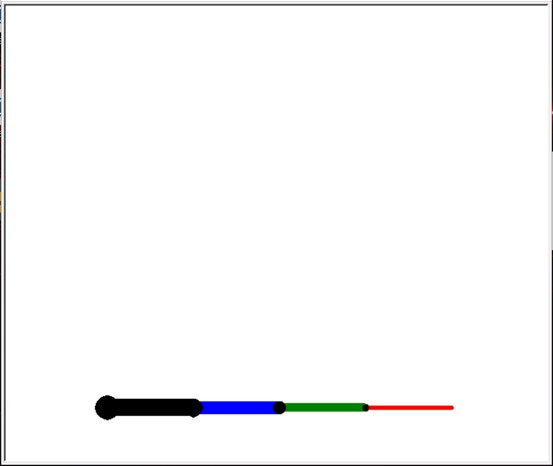
\includegraphics[width=10.5 cm]{Definitions/fig3}
\caption{Moves the terminal to the $(0,400)$ position. \label{fig3}}
\end{figure}   

\subsection{Experimental results of simulation}
In Figure~\ref{fig3}, the robot arm has four links (Link1~Link4). Assuming that the robot arm moves along a straight line, the attitude of each link of the robot arm is calculated by using the particle filter.
We can see the performance of the robot arm by the experimental results as follows. When the robot arm uses the particle filter and the algorithm combined with a large number of random sample points and importance weights, it is obvious that the operation process of the arm is relatively smooth and smooth, and no oscillation occurs.

\begin{figure}[H]
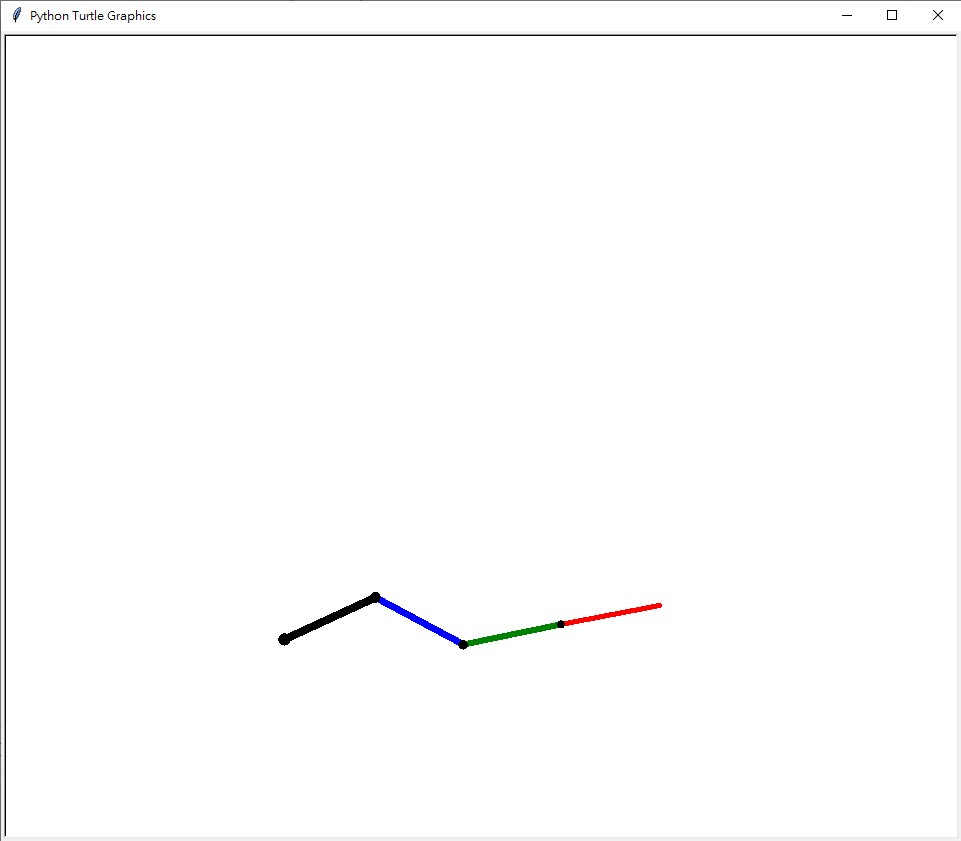
\includegraphics[width=10.5 cm]{Definitions/fig4}
\caption{Arm start point operation. \label{fig4}}
\end{figure}   

\begin{figure}[H]
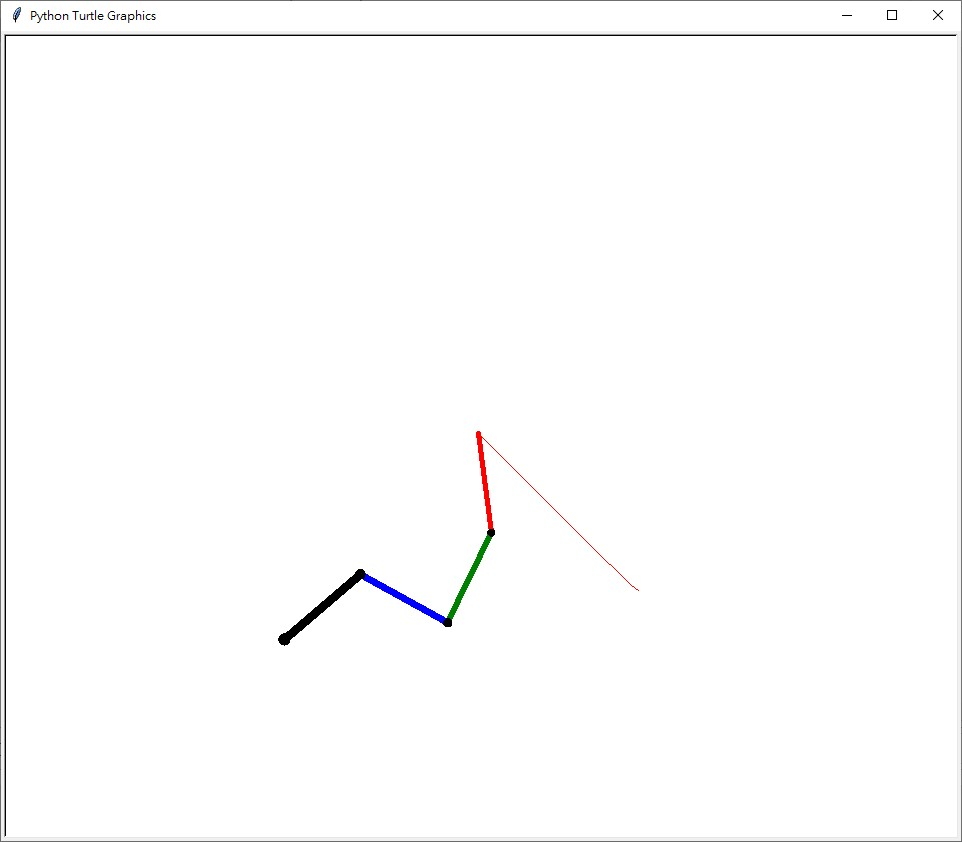
\includegraphics[width=10.5 cm]{Definitions/fig5}
\caption{Arm operation to the center point. \label{fig5}}
\end{figure}   

\begin{figure}[H]
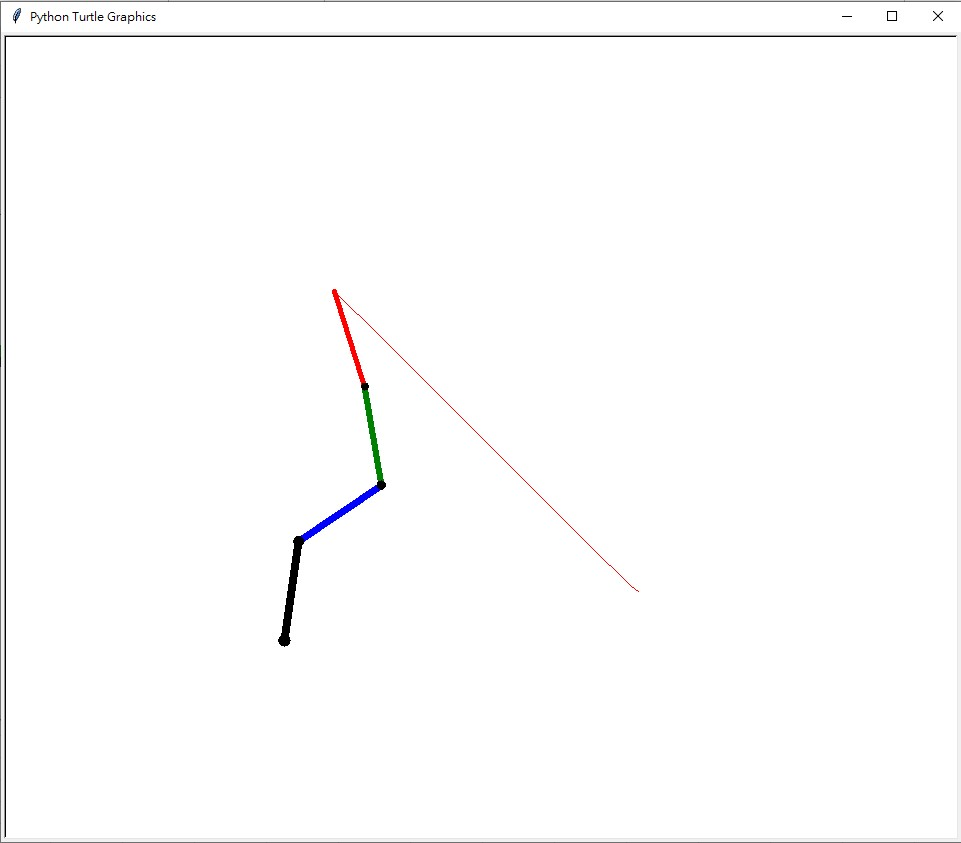
\includegraphics[width=10.5 cm]{Definitions/fig6}
\caption{Arm operation to the end. \label{fig6}}
\end{figure}   

\begin{figure}[H]
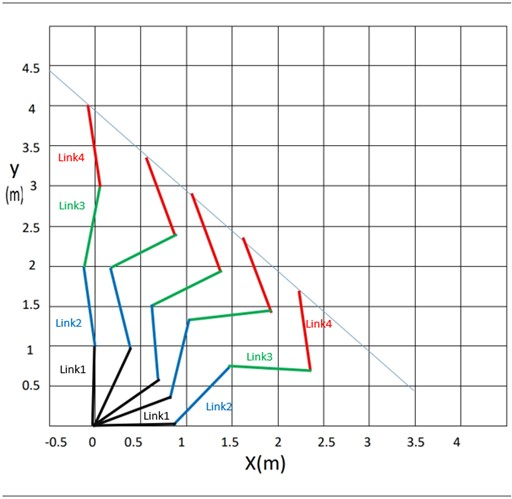
\includegraphics[width=10.5 cm]{Definitions/fig7}
\caption{Movement of the arm in different positions. \label{fig7}}
\end{figure}   


%%%%%%%%%%%%%%%%%%%%%%%%%%%%%%%%%%%%%%%%%%
\section{Conclusions}

A common problem encountered in the inverse kinematics of mechanical arms is the problem of multiple solutions. The multiple solutions often appear symmetrically. In order to avoid the interference of symmetric multiple solutions, we abandon the traditional algebraic or geometric inverse kinematics approach and adopt the Monte Carlo-based nonparametric Bayesian filter (also known as particle filter) to deal with the inverse kinematics problem of robotic arm. The particle filter is designed with a large number of random sample points and importance weights to allow the sample points to converge to the best solution in an iterative process. This paper illustrates how to use the importance weight design to avoid the oscillation problem of symmetric multiple solutions in the adjacent time samples during the robot motion.
Future goals for robotic arms operating in three dimensions are bound to be needed for future research work, and we will be working toward solving the problem of robotic arms in three dimensions.




%%%%%%%%%%%%%%%%%%%%%%%%%%%%%%%%%%%%%%%%%%
\begin{adjustwidth}{-\extralength}{0cm}
%\printendnotes[custom] % Un-comment to print a list of endnotes

\reftitle{References}

% Please provide either the correct journal abbreviation (e.g. according to the “List of Title Word Abbreviations” http://www.issn.org/services/online-services/access-to-the-ltwa/) or the full name of the journal.
% Citations and References in Supplementary files are permitted provided that they also appear in the reference list here. 

%=====================================
% References, variant A: external bibliography
%=====================================
%\bibliography{your_external_BibTeX_file}

%=====================================
% References, variant B: internal bibliography
%=====================================
\begin{thebibliography}{999}
% Reference 1
\bibitem[Author1(year)]{ref-journal1}
Goldenberg, A.A.; Benhabib, B.; Fenton, R.G. A complete generalized solution to the inverse kinematics of robots. {\em IEEE Journal on Robotics and Automation} {\bf 1985}, {\em 1.1}, 14--20.
% Reference 2
\bibitem[Author2(year)]{ref-journal2}
D'Souza, A.; Vijayakumar, S.; Schaal, S. Learning inverse kinematics. {\em Proceedings 2001 IEEE/RSJ International Conference on Expanding the Societal Role of Robotics in the Next Millennium (Cat. No. 01CH37180)} {\bf 2001}, {\em 1}.
% Reference 3
\bibitem[Author3(year)]{ref-journal3}
Kostic, D. et al. Modeling and identification for high-performance robot control: an RRR-robotic arm case study. {\em IEEE Transactions on Control Systems Technology} {\bf 2004}, {\em 12.6}, 904--919.
% Reference 4
\bibitem[Author4(year)]{ref-journal4}
Hou, Z. Geometric method for global stability of discrete population models. {\em Discrete and Continuous Dynamical Systems-B} {\bf 2020}.
% Reference 5
\bibitem[Author5(year)]{ref-journal5}
Falgout, R.D. An introduction to algebraic multigrid. {\em Computing in Science and Engineering} {\bf 2006}, {\em 8}.
% Reference 6
\bibitem[Author6(year)]{ref-journal6}
Jouin, M. et al. Particle filter-based prognostics: review, discussion and perspectives. {\em mechanical systems and signal processing} {\bf 2016}, {\em 72-73},2--31.
% Reference 7
\bibitem[Author7(year)]{ref-journal7}
Mochnac, J.; Marchevsky, S.; Kocan, P. Bayesian filtering techniques: Kalman and extended Kalman filter basics. {\em 2009 19th International Conference Radioelektronika} {\bf 2009}.
% Reference 8
\bibitem[Author8(year)]{ref-book1}
Labbe, R.R.  \textit{Kalman and bayesian filters in python},2014; pp. 43--63.
% Reference 9
\bibitem[Author9(year)]{ref-journal8}
Birgé, L.; Massart, P. Gaussian model selection. {\em Journal of the European Mathematical Society} {\bf 2001}, {\em 3.3}, 203--268.
% Reference 10
\bibitem[Author10(year)]{ref-journal9}
Jiang, Z. et al. A new kind of accurate calibration method for robotic kinematic parameters based on the extended Kalman and particle filter algorithm. {\em IEEE Transactions on Industrial Electronics} {\bf 2017}, {\em 65}.
% Reference 11
\bibitem[Author11(year)]{ref-journal10}
Junior, J. et al. FRPSO: Inverse kinematics using fully resampled particle swarm optimization. {\em 2018 Latin American Robotic Symposium, 2018 Brazilian Symposium on Robotics (SBR) and 2018 Workshop on Robotics in Education (WRE)} {\bf 2018}.










\end{thebibliography}
% If authors have biography, please use the format below
%\section*{Short Biography of Authors}
%\bio
%{\raisebox{-0.35cm}{\includegraphics[width=3.5cm,height=5.3cm,clip,keepaspectratio]{Definitions/author1.pdf}}}
%{\textbf{Firstname Lastname} Biography of first author}
%
%\bio
%{\raisebox{-0.35cm}{\includegraphics[width=3.5cm,height=5.3cm,clip,keepaspectratio]{Definitions/author2.jpg}}}
%{\textbf{Firstname Lastname} Biography of second author}

% For the MDPI journals use author-date citation, please follow the formatting guidelines on http://www.mdpi.com/authors/references
% To cite two works by the same author: \citeauthor{ref-journal-1a} (\citeyear{ref-journal-1a}, \citeyear{ref-journal-1b}). This produces: Whittaker (1967, 1975)
% To cite two works by the same author with specific pages: \citeauthor{ref-journal-3a} (\citeyear{ref-journal-3a}, p. 328; \citeyear{ref-journal-3b}, p.475). This produces: Wong (1999, p. 328; 2000, p. 475)

%%%%%%%%%%%%%%%%%%%%%%%%%%%%%%%%%%%%%%%%%%
%% for journal Sci
%\reviewreports{\\
%Reviewer 1 comments and authors’ response\\
%Reviewer 2 comments and authors’ response\\
%Reviewer 3 comments and authors’ response
%}
%%%%%%%%%%%%%%%%%%%%%%%%%%%%%%%%%%%%%%%%%%
\end{adjustwidth}
\end{document}

